\documentclass[11pt,]{article}
\usepackage[left=1in,top=1in,right=1in,bottom=1in]{geometry}
\newcommand*{\authorfont}{\fontfamily{phv}\selectfont}
\usepackage[]{mathpazo}


  \usepackage[T1]{fontenc}
  \usepackage[utf8]{inputenc}



\usepackage{abstract}
\renewcommand{\abstractname}{}    % clear the title
\renewcommand{\absnamepos}{empty} % originally center

\renewenvironment{abstract}
 {{%
    \setlength{\leftmargin}{0mm}
    \setlength{\rightmargin}{\leftmargin}%
  }%
  \relax}
 {\endlist}

\makeatletter
\def\@maketitle{%
  \newpage
%  \null
%  \vskip 2em%
%  \begin{center}%
  \let \footnote \thanks
    {\fontsize{18}{20}\selectfont\raggedright  \setlength{\parindent}{0pt} \@title \par}%
}
%\fi
\makeatother




\setcounter{secnumdepth}{0}

\usepackage{color}
\usepackage{fancyvrb}
\newcommand{\VerbBar}{|}
\newcommand{\VERB}{\Verb[commandchars=\\\{\}]}
\DefineVerbatimEnvironment{Highlighting}{Verbatim}{commandchars=\\\{\}}
% Add ',fontsize=\small' for more characters per line
\usepackage{framed}
\definecolor{shadecolor}{RGB}{248,248,248}
\newenvironment{Shaded}{\begin{snugshade}}{\end{snugshade}}
\newcommand{\AlertTok}[1]{\textcolor[rgb]{0.94,0.16,0.16}{#1}}
\newcommand{\AnnotationTok}[1]{\textcolor[rgb]{0.56,0.35,0.01}{\textbf{\textit{#1}}}}
\newcommand{\AttributeTok}[1]{\textcolor[rgb]{0.77,0.63,0.00}{#1}}
\newcommand{\BaseNTok}[1]{\textcolor[rgb]{0.00,0.00,0.81}{#1}}
\newcommand{\BuiltInTok}[1]{#1}
\newcommand{\CharTok}[1]{\textcolor[rgb]{0.31,0.60,0.02}{#1}}
\newcommand{\CommentTok}[1]{\textcolor[rgb]{0.56,0.35,0.01}{\textit{#1}}}
\newcommand{\CommentVarTok}[1]{\textcolor[rgb]{0.56,0.35,0.01}{\textbf{\textit{#1}}}}
\newcommand{\ConstantTok}[1]{\textcolor[rgb]{0.00,0.00,0.00}{#1}}
\newcommand{\ControlFlowTok}[1]{\textcolor[rgb]{0.13,0.29,0.53}{\textbf{#1}}}
\newcommand{\DataTypeTok}[1]{\textcolor[rgb]{0.13,0.29,0.53}{#1}}
\newcommand{\DecValTok}[1]{\textcolor[rgb]{0.00,0.00,0.81}{#1}}
\newcommand{\DocumentationTok}[1]{\textcolor[rgb]{0.56,0.35,0.01}{\textbf{\textit{#1}}}}
\newcommand{\ErrorTok}[1]{\textcolor[rgb]{0.64,0.00,0.00}{\textbf{#1}}}
\newcommand{\ExtensionTok}[1]{#1}
\newcommand{\FloatTok}[1]{\textcolor[rgb]{0.00,0.00,0.81}{#1}}
\newcommand{\FunctionTok}[1]{\textcolor[rgb]{0.00,0.00,0.00}{#1}}
\newcommand{\ImportTok}[1]{#1}
\newcommand{\InformationTok}[1]{\textcolor[rgb]{0.56,0.35,0.01}{\textbf{\textit{#1}}}}
\newcommand{\KeywordTok}[1]{\textcolor[rgb]{0.13,0.29,0.53}{\textbf{#1}}}
\newcommand{\NormalTok}[1]{#1}
\newcommand{\OperatorTok}[1]{\textcolor[rgb]{0.81,0.36,0.00}{\textbf{#1}}}
\newcommand{\OtherTok}[1]{\textcolor[rgb]{0.56,0.35,0.01}{#1}}
\newcommand{\PreprocessorTok}[1]{\textcolor[rgb]{0.56,0.35,0.01}{\textit{#1}}}
\newcommand{\RegionMarkerTok}[1]{#1}
\newcommand{\SpecialCharTok}[1]{\textcolor[rgb]{0.00,0.00,0.00}{#1}}
\newcommand{\SpecialStringTok}[1]{\textcolor[rgb]{0.31,0.60,0.02}{#1}}
\newcommand{\StringTok}[1]{\textcolor[rgb]{0.31,0.60,0.02}{#1}}
\newcommand{\VariableTok}[1]{\textcolor[rgb]{0.00,0.00,0.00}{#1}}
\newcommand{\VerbatimStringTok}[1]{\textcolor[rgb]{0.31,0.60,0.02}{#1}}
\newcommand{\WarningTok}[1]{\textcolor[rgb]{0.56,0.35,0.01}{\textbf{\textit{#1}}}}

\usepackage{graphicx,grffile}
\makeatletter
\def\maxwidth{\ifdim\Gin@nat@width>\linewidth\linewidth\else\Gin@nat@width\fi}
\def\maxheight{\ifdim\Gin@nat@height>\textheight\textheight\else\Gin@nat@height\fi}
\makeatother
% Scale images if necessary, so that they will not overflow the page
% margins by default, and it is still possible to overwrite the defaults
% using explicit options in \includegraphics[width, height, ...]{}
\setkeys{Gin}{width=\maxwidth,height=\maxheight,keepaspectratio}

\title{NISS Data Challenge - Education, Employment, and Earnings  }



\author{\Large Nathan Nguyen\vspace{0.05in} \newline\normalsize\emph{Duke University}  }


\date{}

\usepackage{titlesec}

\titleformat*{\section}{\normalsize\bfseries}
\titleformat*{\subsection}{\normalsize\itshape}
\titleformat*{\subsubsection}{\normalsize\itshape}
\titleformat*{\paragraph}{\normalsize\itshape}
\titleformat*{\subparagraph}{\normalsize\itshape}


\usepackage{natbib}
\bibliographystyle{apsr}
\usepackage[strings]{underscore} % protect underscores in most circumstances



\newtheorem{hypothesis}{Hypothesis}
\usepackage{setspace}

\makeatletter
\@ifpackageloaded{hyperref}{}{%
\ifxetex
  \PassOptionsToPackage{hyphens}{url}\usepackage[setpagesize=false, % page size defined by xetex
              unicode=false, % unicode breaks when used with xetex
              xetex]{hyperref}
\else
  \PassOptionsToPackage{hyphens}{url}\usepackage[unicode=true]{hyperref}
\fi
}

\@ifpackageloaded{color}{
    \PassOptionsToPackage{usenames,dvipsnames}{color}
}{%
    \usepackage[usenames,dvipsnames]{color}
}
\makeatother
\hypersetup{breaklinks=true,
            bookmarks=true,
            pdfauthor={Nathan Nguyen (Duke University)},
             pdfkeywords = {},  
            pdftitle={NISS Data Challenge - Education, Employment, and Earnings},
            colorlinks=true,
            citecolor=blue,
            urlcolor=blue,
            linkcolor=magenta,
            pdfborder={0 0 0}}
\urlstyle{same}  % don't use monospace font for urls

% set default figure placement to htbp
\makeatletter
\def\fps@figure{htbp}
\makeatother



% add tightlist ----------
\providecommand{\tightlist}{%
\setlength{\itemsep}{0pt}\setlength{\parskip}{0pt}}

\begin{document}
	
% \pagenumbering{arabic}% resets `page` counter to 1 
%
% \maketitle

{% \usefont{T1}{pnc}{m}{n}
\setlength{\parindent}{0pt}
\thispagestyle{plain}
{\fontsize{18}{20}\selectfont\raggedright 
\maketitle  % title \par  

}

{
   \vskip 13.5pt\relax \normalsize\fontsize{11}{12} 
\textbf{\authorfont Nathan Nguyen} \hskip 15pt \emph{\small Duke University}   

}

}








\begin{abstract}

    \hbox{\vrule height .2pt width 39.14pc}

    \vskip 8.5pt % \small 

\noindent The location of the school where the ninth-graders attended might
contribute to their predicted/aspired future occupation. Different
locations such as the town, city, rural might sociologically affect
one's decision to get a job. To investigate other perspectives in the
original data given by the NISS competition organizer, I use the
variables S4JobIndustry and X4LOCALE to estimate the percentage of
ninth-graders in different high school locations, grouped by 2016
expected occupation.


    \hbox{\vrule height .2pt width 39.14pc}


\end{abstract}


\vskip 6.5pt


\noindent  \begin{Shaded}
\begin{Highlighting}[]
\CommentTok{#load data}
\NormalTok{data <-}\StringTok{ }\KeywordTok{read.csv}\NormalTok{(}\StringTok{"data/HSLSEEESAID.csv"}\NormalTok{)}
\end{Highlighting}
\end{Shaded}

\hypertarget{question-how-did-2009-ninth-graders-attending-high-school-in-different-regions-predict-their-occupation-in-2016}{%
\section{Question: How did 2009 ninth-graders attending high school in
different regions predict their occupation in
2016?}\label{question-how-did-2009-ninth-graders-attending-high-school-in-different-regions-predict-their-occupation-in-2016}}

\begin{Shaded}
\begin{Highlighting}[]
\CommentTok{#load packages and themes}
\KeywordTok{library}\NormalTok{(showtext)}
\KeywordTok{library}\NormalTok{(tidyverse)}
\KeywordTok{library}\NormalTok{(viridis)}
\KeywordTok{font_add_google}\NormalTok{(}\StringTok{"Lora"}\NormalTok{, }\StringTok{"Lora"}\NormalTok{)}
\KeywordTok{showtext_auto}\NormalTok{()}
\end{Highlighting}
\end{Shaded}

\begin{Shaded}
\begin{Highlighting}[]
\NormalTok{order <-}\StringTok{ }\KeywordTok{c}\NormalTok{(}\StringTok{"Don't Know"}\NormalTok{, }\StringTok{"Other"}\NormalTok{, }\StringTok{"Trades and }\CharTok{\textbackslash{}n}\StringTok{ technical"}\NormalTok{, }\StringTok{"STEM"}\NormalTok{, }\StringTok{"Service"}\NormalTok{,}
            \StringTok{"Military and }\CharTok{\textbackslash{}n}\StringTok{ protective services"}\NormalTok{, }\StringTok{"Healthcare"}\NormalTok{, }\StringTok{"Education"}\NormalTok{, }
            \StringTok{"Business and }\CharTok{\textbackslash{}n}\StringTok{ Management"}\NormalTok{, }\StringTok{"Arts and }\CharTok{\textbackslash{}n}\StringTok{ entertainment"}\NormalTok{)}
\end{Highlighting}
\end{Shaded}

\begin{Shaded}
\begin{Highlighting}[]
\CommentTok{#Processing S4JobIndustry's values so that it saves space in the graph}
\NormalTok{data <-}\StringTok{ }\NormalTok{data }\OperatorTok
\StringTok{  }\KeywordTok{mutate}\NormalTok{(}\DataTypeTok{S4JobIndustry =} \KeywordTok{case_when}\NormalTok{(}
\NormalTok{    S4JobIndustry }\OperatorTok{==}\StringTok{ "Military and protective services"} \OperatorTok{~}\StringTok{ }
\StringTok{      "Military and }\CharTok{\textbackslash{}n}\StringTok{ protective services"}\NormalTok{,}
\NormalTok{    S4JobIndustry }\OperatorTok{==}\StringTok{ "Business and Management"} \OperatorTok{~}\StringTok{ }
\StringTok{      "Business and }\CharTok{\textbackslash{}n}\StringTok{ Management"}\NormalTok{,}
\NormalTok{    S4JobIndustry }\OperatorTok{==}\StringTok{ "Arts and entertainment"} \OperatorTok{~}\StringTok{ }
\StringTok{      "Arts and }\CharTok{\textbackslash{}n}\StringTok{ entertainment"}\NormalTok{,}
\NormalTok{    S4JobIndustry }\OperatorTok{==}\StringTok{ "Trades and technical"} \OperatorTok{~}
\StringTok{      "Trades and }\CharTok{\textbackslash{}n}\StringTok{ technical"}\NormalTok{,}
    \OtherTok{TRUE} \OperatorTok{~}\StringTok{ }\NormalTok{S4JobIndustry}
\NormalTok{  ))}
\end{Highlighting}
\end{Shaded}

\begin{Shaded}
\begin{Highlighting}[]
\CommentTok{#process data }
\NormalTok{processed_data <-}\StringTok{ }\NormalTok{data }\OperatorTok
\StringTok{  }\KeywordTok{mutate}\NormalTok{(}\DataTypeTok{S4JobIndustry =} \KeywordTok{factor}\NormalTok{(S4JobIndustry, }\DataTypeTok{levels =}\NormalTok{ order)) }\OperatorTok
\StringTok{  }\KeywordTok{group_by}\NormalTok{(S4JobIndustry, X4LOCALE) }\OperatorTok
\StringTok{  }\KeywordTok{summarise}\NormalTok{(}\DataTypeTok{count_location =} \KeywordTok{n}\NormalTok{()) }\OperatorTok
\StringTok{  }\KeywordTok{group_by}\NormalTok{(S4JobIndustry) }\OperatorTok
\StringTok{  }\KeywordTok{mutate}\NormalTok{(}\DataTypeTok{count =} \KeywordTok{sum}\NormalTok{(count_location)) }\OperatorTok
\StringTok{  }\KeywordTok{mutate}\NormalTok{(}\DataTypeTok{percent =}\NormalTok{ count_location}\OperatorTok{/}\NormalTok{count}\OperatorTok{*}\DecValTok{100}\NormalTok{) }\OperatorTok
\StringTok{  }\KeywordTok{ungroup}\NormalTok{()}

\CommentTok{#create a new variable for positions of percentages on the graphs}
\NormalTok{processed_data <-}\StringTok{ }\NormalTok{processed_data }\OperatorTok
\StringTok{  }\KeywordTok{group_by}\NormalTok{(S4JobIndustry) }\OperatorTok
\StringTok{  }\KeywordTok{mutate}\NormalTok{(}\DataTypeTok{pos =} \DecValTok{100} \OperatorTok{-}\StringTok{ }\KeywordTok{cumsum}\NormalTok{(percent) }\OperatorTok{+}\StringTok{ }\NormalTok{(}\FloatTok{0.5}\OperatorTok{*}\NormalTok{percent))}
\end{Highlighting}
\end{Shaded}

\begin{Shaded}
\begin{Highlighting}[]
\CommentTok{#visualizing with a stacked bar chart}
\NormalTok{g <-}\StringTok{ }\KeywordTok{ggplot}\NormalTok{(processed_data, }\KeywordTok{aes}\NormalTok{(}\DataTypeTok{x =} \KeywordTok{factor}\NormalTok{(S4JobIndustry, }\DataTypeTok{levels =}\NormalTok{ order), }
                           \DataTypeTok{y =}\NormalTok{ percent,}
                           \DataTypeTok{fill =}\NormalTok{ X4LOCALE))}\OperatorTok{+}
\StringTok{  }\KeywordTok{geom_bar}\NormalTok{(}\DataTypeTok{stat =} \StringTok{"identity"}\NormalTok{, }\DataTypeTok{width =} \FloatTok{.5}\NormalTok{)}\OperatorTok{+}
\StringTok{  }\KeywordTok{coord_flip}\NormalTok{()}\OperatorTok{+}\StringTok{ }\CommentTok{#flip the chart}
\StringTok{  }\KeywordTok{scale_fill_manual}\NormalTok{(}\DataTypeTok{values =} \KeywordTok{c}\NormalTok{(}\StringTok{"red"}\NormalTok{, }\StringTok{"black"}\NormalTok{, }\StringTok{"blue"}\NormalTok{, }\StringTok{"grey50"}\NormalTok{))}\OperatorTok{+}\StringTok{ }\CommentTok{#set color}
\StringTok{  }\KeywordTok{theme_linedraw}\NormalTok{()}\OperatorTok{+}
\StringTok{  }\KeywordTok{labs}\NormalTok{(}\DataTypeTok{y =} \StringTok{"Percentage"}\NormalTok{,}
       \DataTypeTok{x =} \StringTok{"Expected Job"}\NormalTok{,}
       \DataTypeTok{fill =} \StringTok{"Location"}\NormalTok{)}\OperatorTok{+}
\StringTok{  }\KeywordTok{theme}\NormalTok{( }\CommentTok{#set theme}
    \DataTypeTok{text =} \KeywordTok{element_text}\NormalTok{(}\DataTypeTok{family =} \StringTok{"Lora"}\NormalTok{, }\DataTypeTok{size =} \DecValTok{12}\NormalTok{),}
    \DataTypeTok{legend.position =} \StringTok{"bottom"}\NormalTok{,}
    \DataTypeTok{panel.grid.major.y =} \KeywordTok{element_blank}\NormalTok{(),}
    \DataTypeTok{panel.grid.minor.x =} \KeywordTok{element_blank}\NormalTok{()}
\NormalTok{  )}\OperatorTok{+}
\StringTok{  }\KeywordTok{scale_y_continuous}\NormalTok{(}\DataTypeTok{labels =} \ControlFlowTok{function}\NormalTok{(x) }\KeywordTok{paste0}\NormalTok{(x, }\StringTok{"%"}\NormalTok{))}\OperatorTok{+}
\StringTok{  }\KeywordTok{geom_text}\NormalTok{(processed_data, }\DataTypeTok{mapping =} \KeywordTok{aes}\NormalTok{(}\DataTypeTok{x =}\NormalTok{ S4JobIndustry, }
                                \DataTypeTok{y =}\NormalTok{ pos,}
                                \DataTypeTok{label =} \KeywordTok{paste0}\NormalTok{(}\KeywordTok{round}\NormalTok{(percent),}\StringTok{"%"}\NormalTok{)), }
            \DataTypeTok{size =} \DecValTok{4}\NormalTok{,}
            \DataTypeTok{color =} \StringTok{"white"}\NormalTok{)}

\NormalTok{g}
\end{Highlighting}
\end{Shaded}

\begin{figure}
\centering
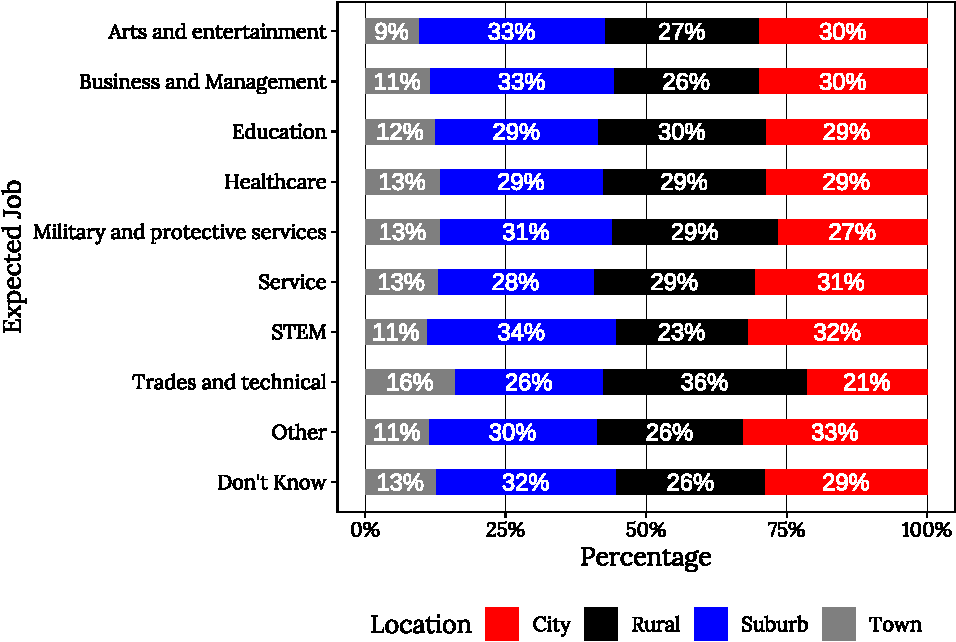
\includegraphics{Nathan-Nguyen-NISS-data-analysis_files/figure-latex/visualization-1.pdf}
\caption{\label{fig:figs}Percentage distribution of 2009 ninth-graders,
by geographical region of last attended high school, grouped by expected
occupations in 2016}
\end{figure}

Based on the visualization, I obtained these key findings:

\begin{itemize}
\tightlist
\item
  Across all the expected occupations, ninth-graders equally attended
  their last high school in city, rural and suburb area, but the
  percentage of ninth-graders attended high school in town is remarkably
  lower (approximately 2 or 2.5 times smaller than the percentage of
  students in city, rural, and suburb area).
\item
  Ninth-graders expected to have an occupation in STEM field tend to be
  on the city and suburb area, with respective percentage of \(32 \%\)
  and \(34 \%\) each, whereas the percentage of ninth-graders in rural
  area and town is remarkably lower compared to the other two (with
  \(23 \%\) and \(11 \%\) each).
\item
  We can see that generally, in each expected occupation, the percentage
  of ninth-graders attended rural high school is slightly lower than the
  percentage of ninth-graders attended their last high school in city
  and suburb. However, we can see that this is not true with the
  expected jobs in trades and technical, education, and service.
\item
  In service, the percentage of ninth-graders attended rural high school
  is slightly lower than the percentage of ninth-graders attended their
  last high school in the suburb (\(29 \%\) compared to \(28 \%\)),
  while considering expected job in education, the percentage of
  ninth-graders attended rural high school is slightly higher than both
  the percentage of ninth-graders attended their last high school in
  city and suburb (\(30 \%\) compared to \(29 \%\) of both city and
  suburb's percentage).
\item
  The most remarkable difference is in the category trades and
  technical, where the percentage of ninth-graders attended rural high
  school is clearly larger than the percentage of ninth-graders attended
  their last high school in city and suburb, which is \(36 \%\),
  remarkably high compared to other category. We can also see that the
  percentage of ninth-graders in town is higher when considering the
  occupation in trades and technical, which is \(16 \%\). It is clear
  that the percentages of ninth-graders expected to have a job in trades
  and technical whose last attended high school is in town and rural
  area, are remarkably higher.
\end{itemize}
\newpage
\singlespacing 
\bibliography{\textasciitilde/Dropbox/master.bib}
\end{document}